\documentclass[%
 %reprint,                 % retiré : l'en-tête d'origine n'utilisait pas reprint
 superscriptaddress,
 amsmath,amssymb,
 aps,
 pra,                      % pre -> pra (comme l'en-tête d'origine)
 floatfix,
]{revtex4-2}

% --- Encoding and language ---
\usepackage[utf8]{inputenc}
\usepackage[T1]{fontenc}
\usepackage[english]{babel}
\usepackage{microtype}
\usepackage{xspace}
\usepackage{xcolor}

% --- Mathematics and symbols ---
\usepackage{mathrsfs, stmaryrd}
\usepackage{amsfonts}
\usepackage{siunitx}
\usepackage{bm}
\DeclareMathOperator\arctanh{arctanh}

% --- Graphics and figures ---
\usepackage{graphicx}
\usepackage{float}        % option [H]
\usepackage{caption}
\usepackage{subcaption}   % si problème avec revtex, utiliser \usepackage{subfig}
\graphicspath{{pictures/}}
\usepackage{placeins}     % pour \FloatBarrier

\captionsetup[figure]{justification=raggedright, singlelinecheck=false, format=plain}
\captionsetup[subfigure]{justification=centering}

% --- Float placement ---
\setcounter{topnumber}{3}
\setcounter{bottomnumber}{3}
\setcounter{totalnumber}{6}
\renewcommand{\topfraction}{0.9}
\renewcommand{\bottomfraction}{0.9}
\renewcommand{\textfraction}{0.1}
\renewcommand{\floatpagefraction}{0.7}
\setlength{\parskip}{0.5\baselineskip}

% --- Tables ---
\usepackage{booktabs}
\usepackage{multirow, array, makecell}
\usepackage{dcolumn}

% --- Lists ---
\usepackage{enumitem}

% --- Algorithms and code ---
\usepackage[ruled,vlined]{algorithm2e}
\usepackage{listings}
\usepackage{fvextra}
\usepackage{tikz}
\usetikzlibrary{decorations.pathreplacing}

% --- Text editing / review ---
\usepackage[normalem]{ulem}
\usepackage{lineno}

% --- References (hyperref avant cleveref) ---
\usepackage{hyperref}
\usepackage{cleveref}
\crefname{algocf}{algorithm}{algorithms}
\Crefname{algocf}{Algorithm}{Algorithms}
\bibliographystyle{apsrev4-2}

% --- Macros : annotations (à retirer avant soumission) ---
\newcommand{\note}[1]{\textcolor{blue}{#1}}
\newcommand{\noteBastien}[1]{\textcolor{blue}{#1}}
\newcommand{\noteMichele}[1]{\textcolor{red}{#1}}
\newcommand{\noteDavid}[1]{\textcolor{green}{#1}}

% --- Macros : code identifiers ---
\newcommand{\UnsignedInt}{\texttt{UnsignedInt}\xspace}
\newcommand{\UnsignedInts}{\texttt{UnsignedInts}\xspace}
\newcommand{\BitSet}{\texttt{BitSet}\xspace}
\newcommand{\BitSets}{\texttt{BitSets}\xspace}
\newcommand{\Bits}{\texttt{Bits}\xspace}

\begin{document}

\linenumbers

\title{Dynamical properties of the Hopfield model\\through bitwise arithmetic}

\author{Bastien Dumont}
 \affiliation{Aix-Marseille Universit\'e, Marseille, France}
 \affiliation{Universit\'e Paris-Saclay, Orsay, France}

\author{David Lacoste}
 \affiliation{Gulliver Laboratory, CNRS UMR 7083, ESPCI Paris, PSL Research University, Paris, France}

\author{Michele Castellana}
 \affiliation{Institut Curie, PSL Research University, CNRS UMR 168, Paris, France}

\date{\today}

%\keywords{Suggested keywords}%Use showkeys class option if keyword
                              %display desired
\maketitle
This document contains additional information to the main paper. The content is summarized in the table of contents below.
\tableofcontents
\section{Method}
We start by presenting the broad implementation of the Metropolis algorithm, before showing how we adapt it to each specific model.


\subsection{Code structure}
We here present the structure of the code. It has been entirely written in \texttt{C++}, taking advantage of the object-oriented structure to factor out the common parts for each model while enabling them to evolve depending on their specificities. Most of the time of this internship has been spent understanding the object-oriented syntax and philosophy, and implementing an easily readable and efficient code for the simulation of the Metropolis algorithm on the different models. The structure found so far is presented in \Cref{fig:architecture}. Once the dynamics is simulated, the outputs are analyzed through python scripts.
\nolinenumbers
\begin{figure}[t]
\centering

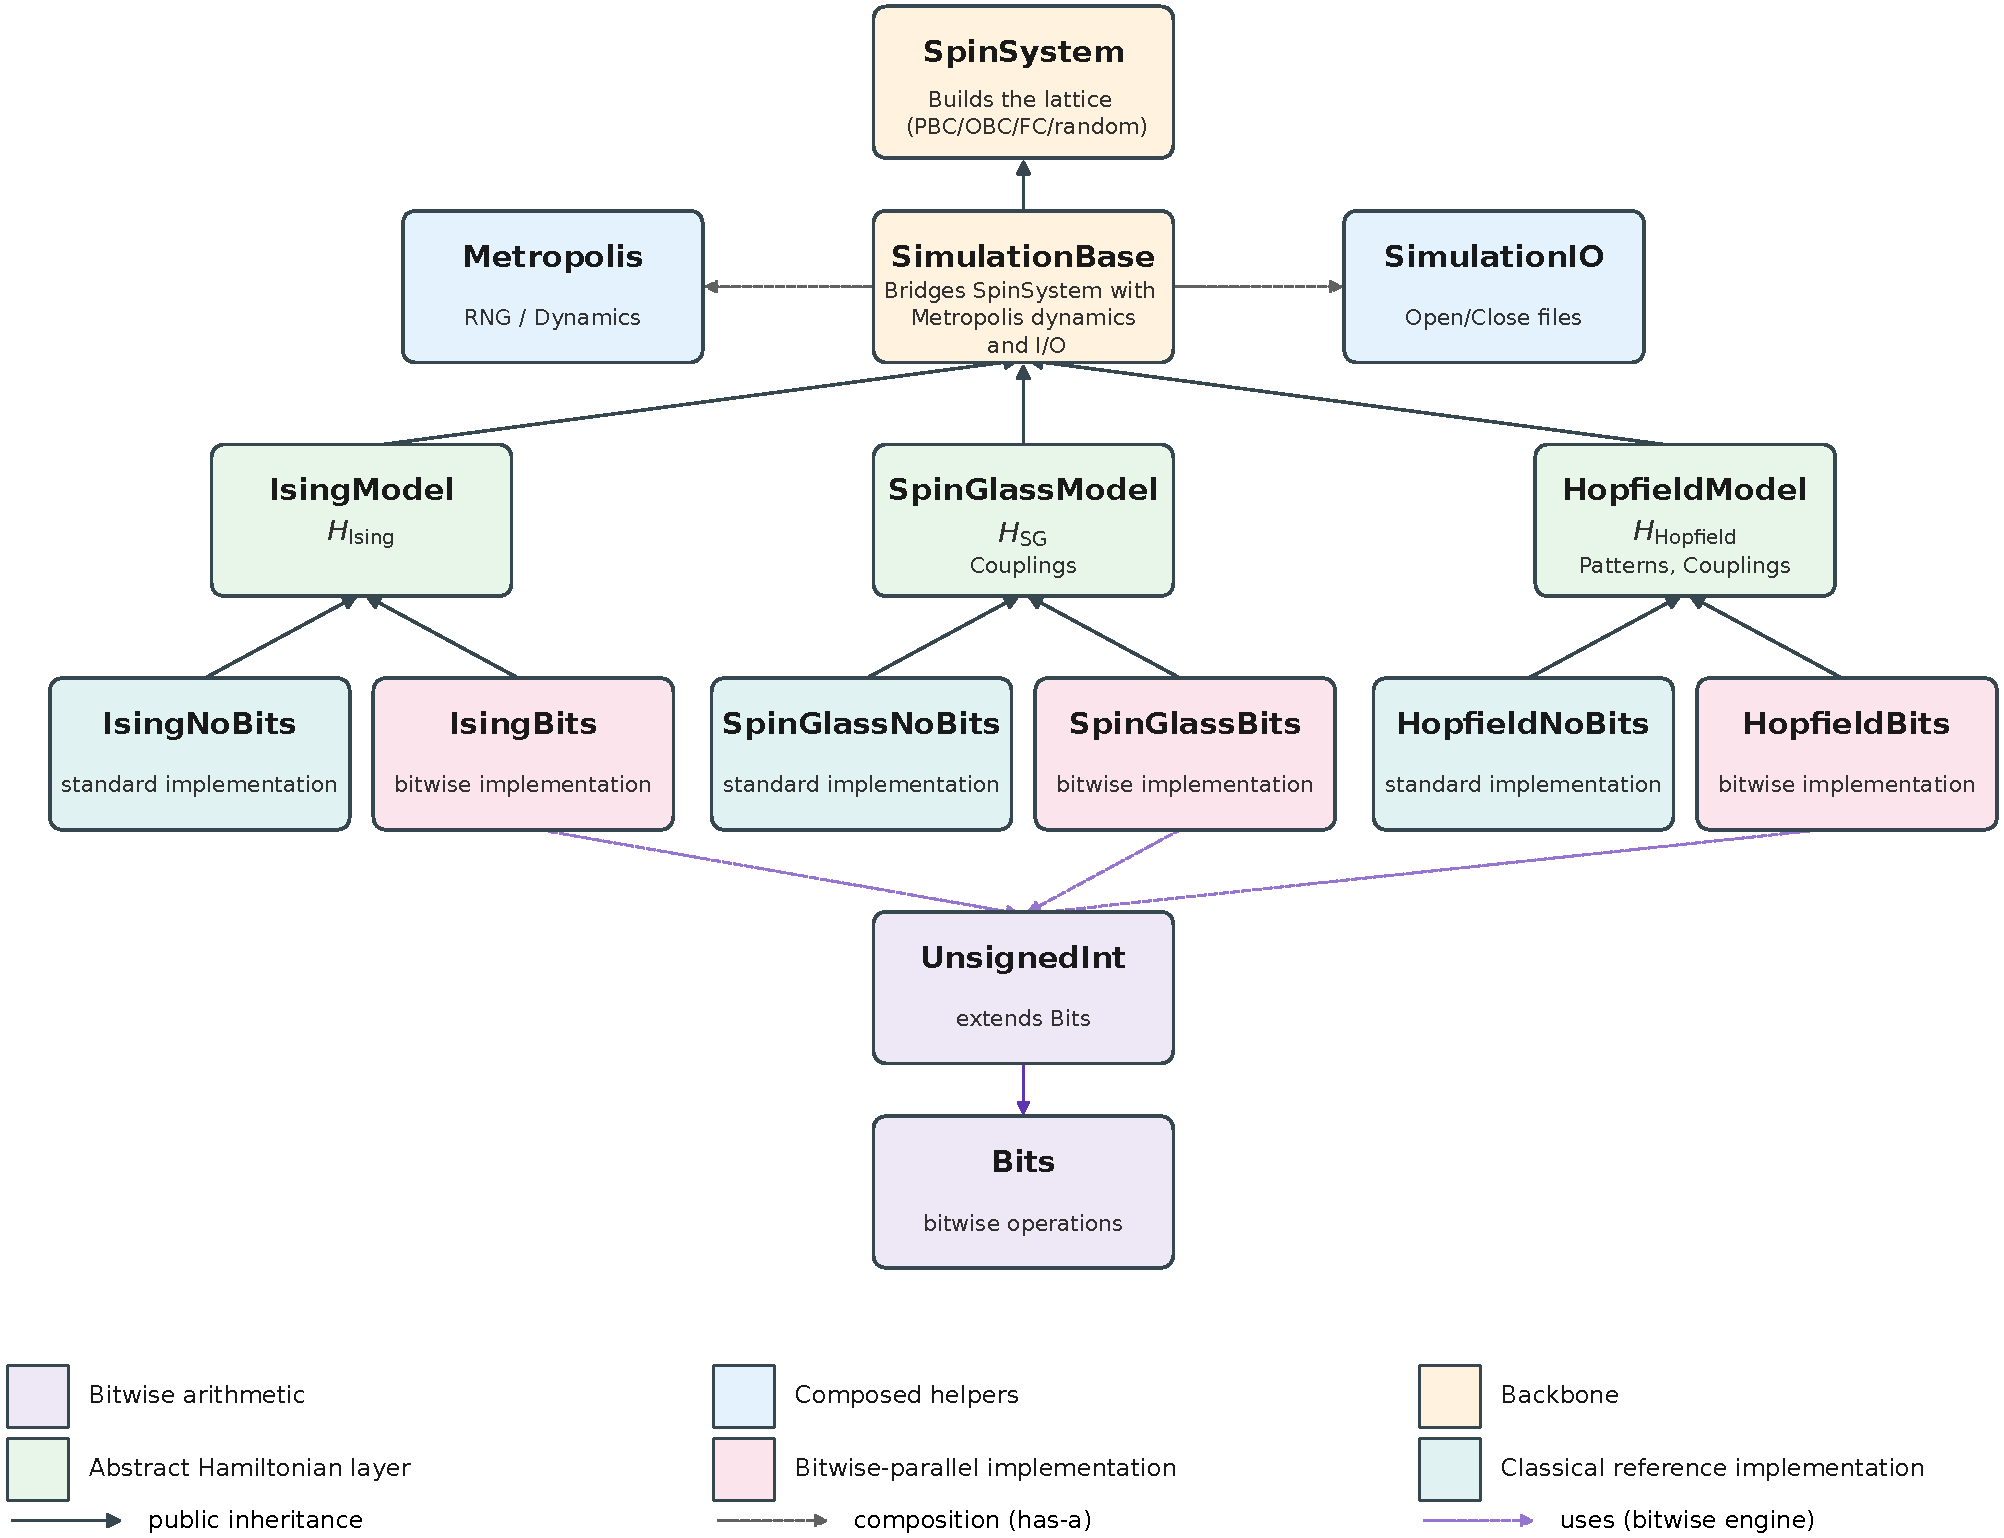
\includegraphics[width=\columnwidth]{architecture.pdf}
\caption{Code structure}
\label{fig:architecture}
\end{figure}
\linenumbers
The code is built around hierarchical classes. We first implement the topology of the network, which is independent of the type of spin interaction and of the dynamical model considered. On this lattice, we set up the evolution rules (\textit{i.e.} the Metropolis algorithm in our case), and the input/output file management. Then, the combination (topology, dynamics) is applied to one of the three models implemented (Ising, Spin glass or Hopfield) and is implemented either in its standard or bitwise version. This code can be found in \cite{hopfield_code}.
\subsection{Naive implementation of the classic Metropolis algorithm}
\nolinenumbers
\begin{algorithm}[b]
\DontPrintSemicolon

\caption{Standard Metropolis implementation  (naive)}

\KwIn{Lattice spins $\{S_i\}$, coupling $J$, inverse temperature $\beta$}
\KwOut{Updated lattice spins $\{S_i\}$}
\BlankLine
\BlankLine
\For{$\mathrm{sweep} = 1$ \KwTo $N_{\mathrm{sweeps}}$}{
    \For{$\mathrm{step}=1$ \KwTo $N$}{
        Draw $k$ among $N$\;
      \For{$r = 1$ \KwTo $n_\text{bits}$}{
          Compute $\Lambda_k^{(r)}$\;
          \BlankLine
          \tcp{Unconditional flip: energy is lowered}
          \eIf{$\Lambda_k^{(r)} \leq 0$}{
              $s_k^{(r)} \leftarrow -s_k^{(r)}$\;
          }{
              \tcp{Conditional flip: draw Poisson threshold}
              Draw $q$ with $\theta \sim \mathcal{E}(\beta \kappa)$\;
              \If{$m \geq \Lambda_k^{(r)}$}{
                  $s_k^{(r)} \leftarrow -s_k^{(r)}$\;
              }
          }
      }
    }
}
\label{alg:ising_classic_naive}
\end{algorithm}
\FloatBarrier
\input{ising}
\FloatBarrier
\section{The Spinglass model}
We now move on a more complex model, in order to approach the structure of the Hopfield network.
\subsection{The Edwards–Anderson model}
The Edwards–Anderson (EA) model -- first introduced by Edwards and Anderson in 1975 \cite{SFEdwards_1975} -- is a finite dimensional spin glass model with short range interaction. It is not a mean field spin glass model with infinite range interactions such as the Sherrington–Kirkpatrick model \cite{SK_model}. The model is formally described as follows:
\begin{equation}
  H_\text{EA}=\sum_{\langle i,j \rangle}J_{ij}S_iS_j.
  \label{eq:EA_model}
\end{equation}
Where $J_{ij}$ is a random variable taking its values in $\{-1,\,1\}$ with equal probability. Thus, it can easily be represented by a \Bits.
Under a spin flip ($S_k \to - S_k$), the energy shift is:
\begin{equation}
  \Delta E_k=2 S_k \sum_{i \in \partial k}J_{ki}S_i.
  \label{eq:DeltaE_EA}
\end{equation}
The structure being really similar to that of \eqref{eq:DeltaE_ising}, we can perform the same derivation as for the Ising model and find the spin flip condition:
\begin{equation}
  \lfloor \rho \rfloor \geq S_k  \sum_{i \in \partial k}J_{ki}S_i,\\
  \label{eq:flip_EA_int}
\end{equation}
with this time $\rho \sim \mathcal{E}(2\beta)$.
\subsection{Bitwise Implementation}
We now need to express the product $J_{ik}S_kS_i$ in a binary way. As shown in the previous section, the product $S_kS_i$ can be re-written $(-1+2B_k)(-1+2B_i)=-1+2 C_{ki}$ with $C_{ki}= B_k \odot B_i$. Thus, by writing $J_{ki}=-1+2K_{ki}$ with $K_{ki}$ a \Bits, we have:
\begin{equation*}
  \begin{aligned}
  J_{ik}S_kS_i =& (-1+2K_{ki})(-1+2 C_{ki})\\
               =& -1 + 2D_{ki},\\
  \end{aligned}
\end{equation*}
with $D_{ki}=K_{ki}\odot C_{ki}= K_{ki} \odot B_k \odot B_i =  K_{ki} \oplus B_k \oplus B_i$. As in the previous section, the flip condition is then:
\begin{equation}
  \lfloor \rho \rfloor + n_k \geq 2 \sum_{i \in \partial k}D_{ki}.
  \label{eq:flip_SG_bitwise}
\end{equation}
Both the bitwise and the classic implementation are thus similar to this of the Ising model, and we will not present them further in this report. The bitwise algorithm for the spin glass model can be found in the appendix, see \Cref{alg:SG_bitwise}.\\
The bitwise implementation is not validated here, as the bitwise framework was already tested in the previous section, and the main interest of this model lies in bridging the complexity gap between the Ising model and the Hopfield network. We nonetheless verified that the standard and the bitwise implementations produce identical spin configurations when initialized from the same initial state and driven by the same sequence of random numbers.
\begin{algorithm}[t]
\DontPrintSemicolon
\caption{Bitwise spin glass Metropolis}

\KwIn{Bit-replicated spins $\{B_i\}$, couplings $\texttt{Couplings}$, neighbor lists $\partial i$, inverse temperature $\beta$}
\KwOut{Updated spin configurations $\{B_i\}$}

\BlankLine
\textbf{Preallocated variables:} $\mathtt{Bits}\ \texttt{xnor},\ \texttt{mask}$\;
\phantom{\textbf{Preallocated variables:}} $\mathtt{UnsignedInt}\ T_i,\ \texttt{threshold}$\;

\BlankLine

\For{$\mathrm{sweep}=1$ \KwTo $N_{\mathrm{sweeps}}$}{
    \For{$\mathrm{step}=1$ \KwTo $N$}{
        Draw $k$ among $N$\;
        Draw $\lfloor \rho \rfloor$ with $\rho \sim \mathcal{E}(2\beta)$

        \eIf{$\lfloor \rho \rfloor \ge n_k$}{
            $B_k \leftarrow \neg B_k$ \tcp*{escape condition: unconditional flip across all replicas}
        }{
            $T_k \leftarrow \mathbf{0}$

            $\mathtt{threshold} \leftarrow \mathbf{0}$

            \For{$i \in \partial k$}{
                $\mathtt{xnor}\ \leftarrow K_{ki} \oplus B_k \oplus B_i$
                \tcp*{bitwise XNOR across replicas}

                $T_k \mathrel{+}= \mathtt{xnor}$
                \tcp*{increment agreement count per replica}
            }

            $T_k \leftarrow 2T_k$

            $\mathtt{threshold} \leftarrow \lfloor \rho \rfloor +n_k$

            $\mathtt{mask} \leftarrow (T_k \le \mathtt{threshold})$
            \tcp*{per-replica flip condition}

        $B_k \leftarrow B_k \oplus \mathtt{mask}$ \tcp*{bitwise spin flip (XOR operation): only replicas}
        \tcp*[r]{for which $\mathtt{mask}^{(\ell)}=1$ are flipped}
        }
    }
}

\label{alg:SG_bitwise}
\end{algorithm}
\FloatBarrier
\subsection{Performance test}
 We now test the performance of the implementation, for several lattice sizes and the temperatures, this time with $N_\text{sweeps}=2^{14}$. The results are shown in \Cref{fig:speedup_spinglass}. We notice the same evolution of the normalized time for both implementation as the ones observed for the Ising model. The shape of the speedup factor is similar to this of the Ising model, but its evolution is steadier, with what appears to be a saturation for the highest temperatures. The time per sweep also remains proportional to the system size, the complexities of the implementations thus should be similar to those of the Ising model.

\clearpage
\newpage
\FloatBarrier


\nolinenumbers
\begin{figure}[htbp]
\centering
% ── Top row ───────────────────────────────────────────────────────────────
\begin{minipage}[b]{0.49\textwidth}
    \centering
    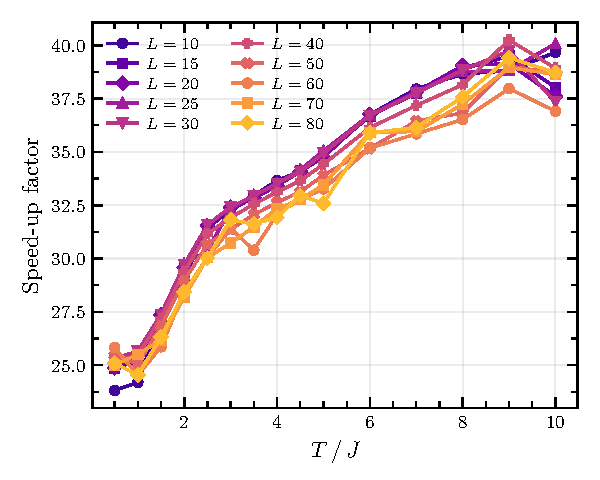
\includegraphics[width=\columnwidth]{speedup_curves_spinglass.pdf}
    \subcaption{Speedup factor evolution.}
    \label{fig:speedup_curve_spinglass}
\end{minipage}
\hfill
\begin{minipage}[b]{0.49\textwidth}
    \centering
    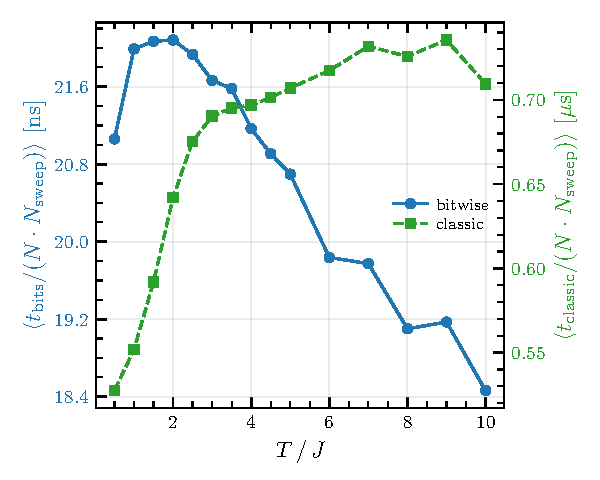
\includegraphics[width=\columnwidth]{time_normalized_spinglass.pdf}
    \subcaption{Normalized time evolution.}
    \label{fig:normalised_time_spinglass}
\end{minipage}

\vspace{0.5em}

% ── Bottom row ────────────────────────────────────────────────────────────
\begin{minipage}[b]{\textwidth}
    \centering
    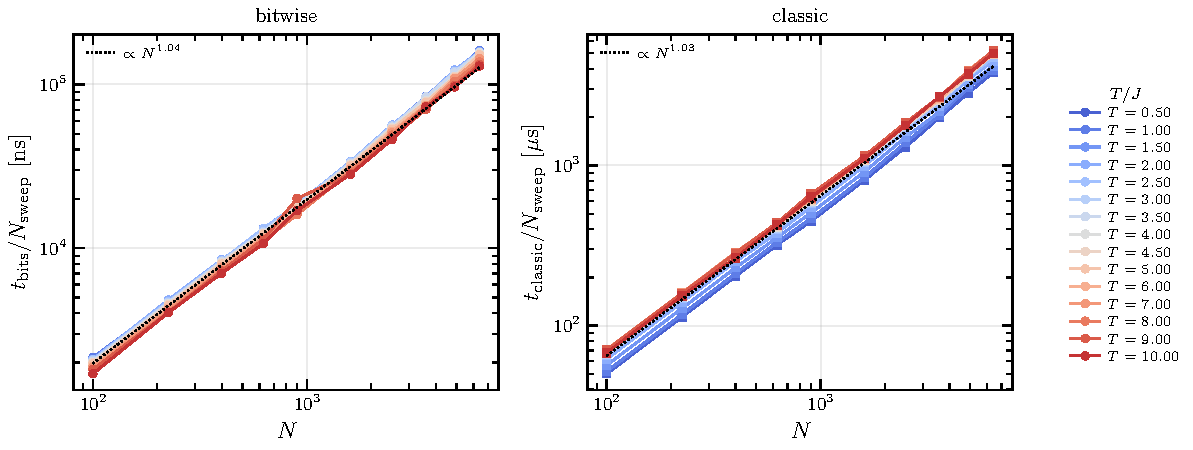
\includegraphics[width=\columnwidth]{time_total_vs_N_spinglass.pdf}
    \subcaption{Sweep time depending on the lattice size for all temperatures.}
    \label{fig:sweep_time_vs_N_spinglass}
\end{minipage}
\caption{Performance analysis of the bitwise and classical Spin Glass Metropolis implementations.}
\label{fig:speedup_spinglass}
\end{figure}
\linenumbers
\FloatBarrier

\FloatBarrier
\section{The Hopfield model}
\subsubsection{Naive implementation}
A first naive implementation would be to unfold $G_{ki}$ into its pattern components in order to deal with \Bits only objects. The flip condition would then be:

\begin{equation}
 q\geq \sum_{i \in \partial k}\sum_{\mu=1}^{p}\xi_k^\mu \xi_i^\mu S_k S_i.
\end{equation}
As seen in the previous sections, the product $\xi_k^\mu \xi_i^\mu S_k S_i$ can simply be expressed from  $X_k^\mu \odot X_i^\mu \odot B_k \odot B_i$, where $X_k^\mu$ is the boolean variable associated with $\xi_k^\mu$. This method presents the advantage to not require too much memory allocation to store the couplings $G_{ki}$ as they are not stored before the evolution but computed on the fly in the hot loop.
However, it requires summing over the patterns, thus introducing  an additional complexity of $\mathcal{O}(p)=\mathcal{O}(\alpha N)$ per spin update, which is done $N \cdot N_\text{sweeps}$ times. This would result in a significant loss of performance.

\begin{algorithm}[b]
\nolinenumbers
\DontPrintSemicolon
\caption{Bitwise Hopfield Metropolis using shifted overlaps}

\KwIn{Bit-replicated spins $\{B_i\}$, patterns $\{X_i^\mu\}$, shifted overlaps $\{\tilde{M}^\mu\}$, shifted couplings $\{\tilde{G}_{ij}\}$, neighbor lists $\partial i$, number of patterns $P$}
\KwOut{Updated spin configurations $\{B_i\}$}

\BlankLine

\textbf{Preallocated variables:}

$\mathtt{Bits}\ C_{ij},\ C_i^\mu,\ \mathtt{mask}$\;

$\mathtt{UnsignedInt}\
\Sigma_C,\
\Sigma_{CM},\
\Sigma_{CG},\
\Sigma_M,\
\mathrm{LHS},\
\mathrm{RHS}$\;

\BlankLine

\For{$\mu=1$ \KwTo $P$}{
    $\Sigma_M\leftarrow\Sigma_M+\tilde{M}^\mu$
}
\tcp*{Precompute shifted overlap sum}

\BlankLine

\For{$i=1$ \KwTo $N$}{
    $\Sigma_G(i)\leftarrow0$\;
    \For{$j\notin\partial i,\ j\neq i$}{
        $\Sigma_G(i)\leftarrow\Sigma_G(i)+\tilde{G}_{ij}$
    }
}
\tcp*{Precompute shifted non-neighbor coupling sums}

\BlankLine

\For{$\mathrm{sweep}=1$ \KwTo $N_{\mathrm{sweeps}}$}{

\For{$\mathrm{step}=1$ \KwTo $N$}{

    Draw random neuron $k$\;

    Draw $q$ with $\theta\sim\mathcal{E}(2\beta)$\;\;


    \eIf{$m \geq p n_k$}{

        \For{$\mu=1$ \KwTo $P$}{

            $C_k^\mu\leftarrow B_k\odot X_k^\mu$\;

            $\tilde{M}^{\mu}
            \leftarrow
            \tilde{M}^{\mu}
            +2-4C_k^\mu$\;
        }
        $\Sigma_M
        \leftarrow
        \Sigma_M
        + 2P
        - 4\sum_{\mu=1}^{P} C_k^\mu$
        \tcp*{Update shifted overlaps}
        $B_k\leftarrow\neg B_k$\;\;

    }{

        $\Sigma_C\leftarrow0$\;

        $\Sigma_{CG}\leftarrow0$\;


        \For{$i\notin\partial k,\ i\neq k$}{

            $C_{ik}\leftarrow B_i\odot B_k$\;

            $\Sigma_C\leftarrow\Sigma_C+C_{ik}$\;

            $\Sigma_{CG}
            \leftarrow
            \Sigma_{CG}
            +C_{ik}\odot\tilde{G}_{ki}$
        }


        $\Sigma_{CM}\leftarrow0$\;

        \For{$\mu=1$ \KwTo $P$}{

            $C_k^\mu\leftarrow B_k\odot X_k^\mu$\;

            $\Sigma_{CM}
            \leftarrow
            \Sigma_{CM}
            +C_k^\mu\odot\tilde{M}^\mu$
        }


        $\mathrm{LHS}
        \leftarrow
        m
        +2N\Sigma_C
        +\Sigma_M
        +2\Sigma_{CG}$\;


        $\mathrm{RHS}
        \leftarrow
        p n_k
        +2\Sigma_{CM}
        +\Sigma_G(k)
        +2p\Sigma_C$\;


        $\mathtt{mask}
        \leftarrow
        (\mathrm{RHS}\leq\mathrm{LHS})$
        \tcp*{Bitwise evaluation of Eq.~\eqref{eq:bitwise_flip_overlap}}


        \For{$\mu=1$ \KwTo $P$}{

            $C_k^\mu
            \leftarrow
            C_k^\mu\land\mathtt{mask}$\;

            $\tilde{M}^{\mu}
            \leftarrow
            \tilde{M}^{\mu}
            +2\mathtt{mask}
            -4C_k^\mu$
        }
        $\Sigma_M \leftarrow \Sigma_M
        + 2P\mathtt{mask}
        - 4\sum_{\mu=1}^{P}C_k^\mu\mathtt{mask}$\;

        $B_k
        \leftarrow
        B_k\oplus\mathtt{mask}$\;
    }
}
}
\label{alg:Hopfield_bitwise_overlaps}
\end{algorithm}
\linenumbers
\FloatBarrier
\bibliographystyle{unsrt}
\bibliography{references}

\end{document}